
\chapter{Aprendizaje Automático}
\label{chap:Aprendizaje-Automatico}

\section{Introducción}
En el contexto de aprendizaje automático, los patrones deben ser descubierto a partir de una serie de ejemplos que son denominados instancias. Tal conjunto de entrada se denomina conjunto de entrenamiento. En nuestro caso específico, cada instancia es un vector de características extraída de señales en una determinada ventana de tiempo. Los ejemplos en el conjunto de entrenamiento pueden o no pueden ser etiquetados, es decir, asociada a una clase conocida (por ejemplo, caminar, correr, etc.). En algunos casos, tener datos etiquetados no es factible, ya que puede requerir un experto para examinar manualmente los ejemplos y asignar una etiqueta en base a su experiencia.

Este proceso es generalmente tedioso, caro y consume mucho tiempo en muchas aplicaciones de minería de datos. Existen dos enfoques de aprendizaje, es decir, aprendizaje supervisado y no supervisado, que se ocupan de datos etiquetados y no etiquetados, respectivamente. Puesto que un sistema de reconocimiento de la actividad humana debe devolver un marcador tal como caminar, sentarse, correr, etc., la mayoría de los sistemas de HAR utilizan modelos de aprendizaje supervisados. De hecho, podría ser muy difícil de discriminar actividades en un contexto completamente sin supervisión. Algunos otros sistemas funcionan de una manera semisupervisada en donde parte de los datos están sin etiqueta.

\section{Aprendizaje supervisado}
El etiquetado de datos detectados a partir de individuos que realizan diferentes actividades es una tarea relativamente fácil.
Algunos sistemas guardan datos del sensor en medios no volátiles mientras que una persona del equipo de investigación supervisa el proceso de recolección y de forma manual registra y etiqueta la actividad en cada intervalo de tiempo. Otros sistemas se caracterizan por una aplicación móvil que permite al usuario seleccionar la actividad que se realiza a partir de una lista, de esta manera, cada muestra se corresponde con una etiqueta de actividad y, a continuación, se almacena en el servidor. Este ultimo utilizado en este trabajo.

El aprendizaje supervisado ha sido un campo muy productivo, dando lugar a un gran número de algoritmos. La Tabla V resume los clasificadores más importantes en el reconocimiento de la actividad humana y su descripción se incluye a continuación.

**insertar listado de algoritmos**

En las siguientes secciones nos concentramos en el árbol de decisión, el cual fue utilizado para este trabajo.

\section{Arboles de Decisión}
El árbol de decisión es un método de aprendizaje predictivo de una conjunto de tuplas o instancias etiquetadas. Un árbol de decisión es una estructura de árbol similar a un diagrama de flujo, donde cada nodo interno (nodo no hoja) denota una prueba de un atributo, y cada rama representa el camino de a seguir luego de la evaluación, y cada nodo hoja es una etiqueta o clase.

\begin{figure}[!htbp]
	\centering
	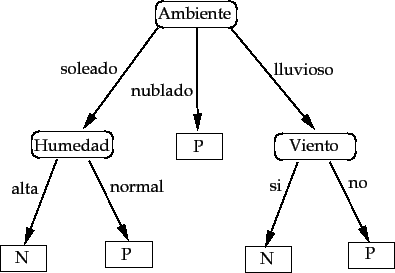
\includegraphics[width=0.7\linewidth]{capitulo-3/graphics/ad_1}
	\caption[Árbol de decisión]{Árbol de decisión}
	\label{fig:arbolEjemplo}
\end{figure}

\section{Algoritmo}

\begin{algorithm}
	\caption{Árbol de Decisión - C4.5}
	\label{algoC45}
	\begin{algorithmic}[1]
		\Require Conjunto de datos etiquetados $D$
		\Procedure{C4.5}{$ D $}
			\If {$D > \textit{es puro o cumple el criterio de parada} $} 
				\State\textit{Termina}
			\EndIf
			\ForAll{$a \in D $}
				\State $\textit{Computar información de division en a }$
			\EndFor
			\State $ a_{best} =$ Mejor atributo de división respecto al criterio 
			\State $ Arbol =$ Crear un nodo de decisión con $ a_{best} $ en la raíz 
			\State $ D_{v} =$ Introducir sub-conjunto de $D$ basado en división $ a_{best} $
			\ForAll{$ D_{v} $}
				\State $ Arbol_{v} = C4.5(D_{v}) $
				\State Unir $ Arbol_{v} $ al correspondiente arco del Árbol
			\EndFor
			\State 
			\Return $ Arbol $
		\EndProcedure
	\end{algorithmic}
\end{algorithm}
